\documentclass[12]{article}
\usepackage{graphicx}
\usepackage{color}
\usepackage{algorithmic}
\begin{document}

\title{\textbf{
\includegraphics[scale=0.5]{42.png}
\textcolor{red}{Universitatea din Craiova \\Facultatea de Automatic\u{a},Calculatoare \c{s}i Electronic\u{a}}}}
\date{\textbf{04 June 2016}}
\maketitle
\begin{center}
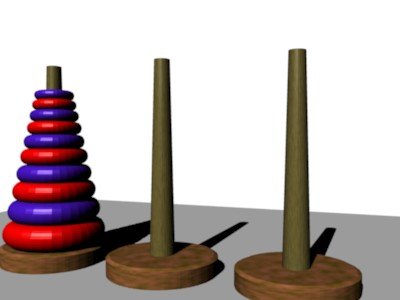
\includegraphics[scale=0.6]{towers-of-hanoi.jpg}
\end{center}
\textbf{Project : Programming Techniques} \\
\textbf{Title : A library for matrix functions}\\
\textbf{Teachers : Becheru Alex \& B\u{a}dic\u{a} Costin \& Murare\c{t}u Ionu\c{t} }\\
\textbf{Student : Negrea Andrei Adelin} \\
\textbf{Section : Calculatoare Rom\^{a}n\u{a}\\ Year I\\ Group : 1.2 B}
\newpage
\tableofcontents


\newpage
\section{Problem Statement}

\textcolor{white}{}
\subsection{Title}
         \textcolor{blue}    {Tower of Hanoi}
\subsection{Description}
\textcolor{white}{}

My project refers to an application that will solve the hanoi towers problem. There are three given rods defined as A,B,C. 
On rod A we have n plates of different diameters,in increasing order of diameters,from top to bottom. Initially rods B and C are empty. 
The application will display all the moves in the next order: plates on the rod A will be moved to rod B,in the same order,using C as a maneuvering rod and respect the following rules: at every step one plate will move; a disk can only be placed over a larger diameter disc.



\newpage
\section{Pseudocode}
\subsection{Read File}
 \begin{algorithmic}[1]
\STATE $START$
\STATE $INT \ i,j,n,m$
 \STATE $FILE  *f$
 \STATE $f=fopen("date.out","a")$
  \STATE $fseek( f , nr * 2 , SEEK\_CUR )$
  \STATE $fprintf(f, "\%d -> \%d ", a, b)$
  \STATE $print("\%d -> \%d ", a, b)$
  \STATE $fclose(f)$
\end{algorithmic}


\subsection{Divide et Impera}
\begin{algorithmic}
\IF{$n$}
    \STATE $hanoi(n-1,a,c,b)$
    \STATE $write( a, b)$
    \STATE $nr++$
    \STATE $hanoi(n-1,c,b,a)$
    \ENDIF
\end{algorithmic}


\subsection{Stack Implementation}

\begin{algorithmic}
\STATE $START$
\STATE $INT \ i$  
\STATE $FILE *out$
\STATE $out = fopen("output.txt","a")$
\FOR{$i = 1$  \TO n}
    \IF{$i > 0$}
     \IF{$i \% 2$}
        \IF{$t \% 2$}
            \STATE $s2 = y$
            \IF{$stack[i] != 0$}
                \STATE $r2 = stack[i]-1$
            \ELSE
                \STATE $r2 = s2$
            \ENDIF
            \IF{$r2 < 1$}
                \STATE $r2 = 3$
            \ENDIF
        \ENDIF
        \ELSE
            \STATE $s2 = y-1$
            \IF{$stack[i] != 0$}
                \STATE $r2 = stack[i]+1$
            \ELSE
                \STATE $r2 = s2$
            \ENDIF
            \IF{$r2 > 3$}
                \STATE $r2 = 1$
            \ENDIF
        \STATE $stack[i] = r2$
        \STATE $printf("Disk \%d move from \%d to \%d",i,x,r2)$
        \STATE $fprintf(out,"Disk \%d move from \%d to \%d",i,x,r2)$
        \STATE $f(i-1, r1, r2)$
        \ENDIF
        \ELSE
            \IF{$t \% 2$}
                \STATE $s1 = y-1$
            \ENDIF
                \IF{$stack[i] != 0$}
                    \STATE $r1 = stack[i]-1$
                \ELSE
                    \STATE $r1 = s1$
                \ENDIF
                \IF{$r1 < 1$}
                    \STATE $r1 = 3$
                \ENDIF
        \STATE $stack[i] = r1$
        \STATE $printf("Disk \%d move from \%d to \%d",i,x,r1)$
        \STATE $fprintf(out ,"Disk \%d move from \%d to \%d",i,x,r1 )$
        \STATE $f(i-1, r2, r1)$
    \ENDIF
\ENDFOR
\STATE $End$
\end{algorithmic}


\newpage
\section{Application Design}
\textbf{}

\subsection{Recursiv function}

In my problem : 

If n = 1,  A$->$B move is made,namely the plate on the rod A moves on rod B. 
If n = 2,  A$->$C , A$->$B, C$->$B moves are made. 
In case of n $>$ 2 , the problem is complicated. 
We will note H(n,a,b,c) the sequence of the n drives moves from rod A to rod B using as a intermediate rod, rod C. 
According to the Divide et Impera strategy, we will try to break the problem in two other subproblems of the same type, then we will combine the solutions. In this case, we observe that the move of the n plates is equivalent to: \\
- n-1 move from rod A to rod C, using rod B \\
- moving the remaining disk on rod B \\
- n-1 move from rod C to rod B, using rod A

\subsection{Input Data}
\textcolor{white}{}

For my problem the input will be n. N is the number of disks and it's introduce from the keyboard in the runscreen. 


\subsection{Output Data}
\textcolor{white}{}

The output data which represents the actual result of the problem step by step will be present in the file output\_method1.txt for the first algorithm and respectively output\_method2.txt for the second algorithm .

\subsection{Functions}
\textcolor{white}{}

The functions used in the program are presented in the \textbf{Section 2}, in their pseudocode forms.

\section{Source Code}

\textcolor{white}{}


My project is called ``Tower of Hanoi.`` . The source code is created in  programming language standard C99, that is compiled in one  compiler.

 The  compiler is in \textcolor{blue}{GNU GCC Compiler} with help program Code Blocks 16. 

\section{Experiments and results}
\textcolor{white}{}
\subsection{GNU GCC Compiler}

Method1

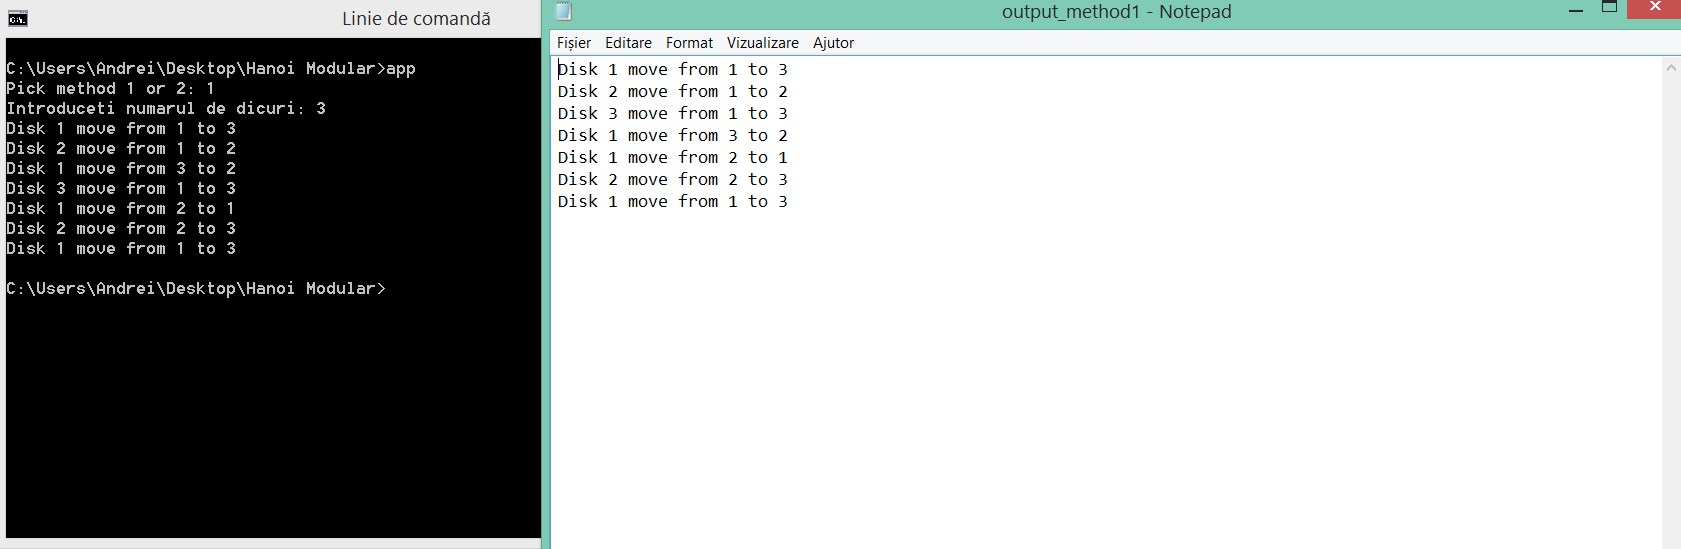
\includegraphics[scale=0.4]{metoda1.png}

Method2

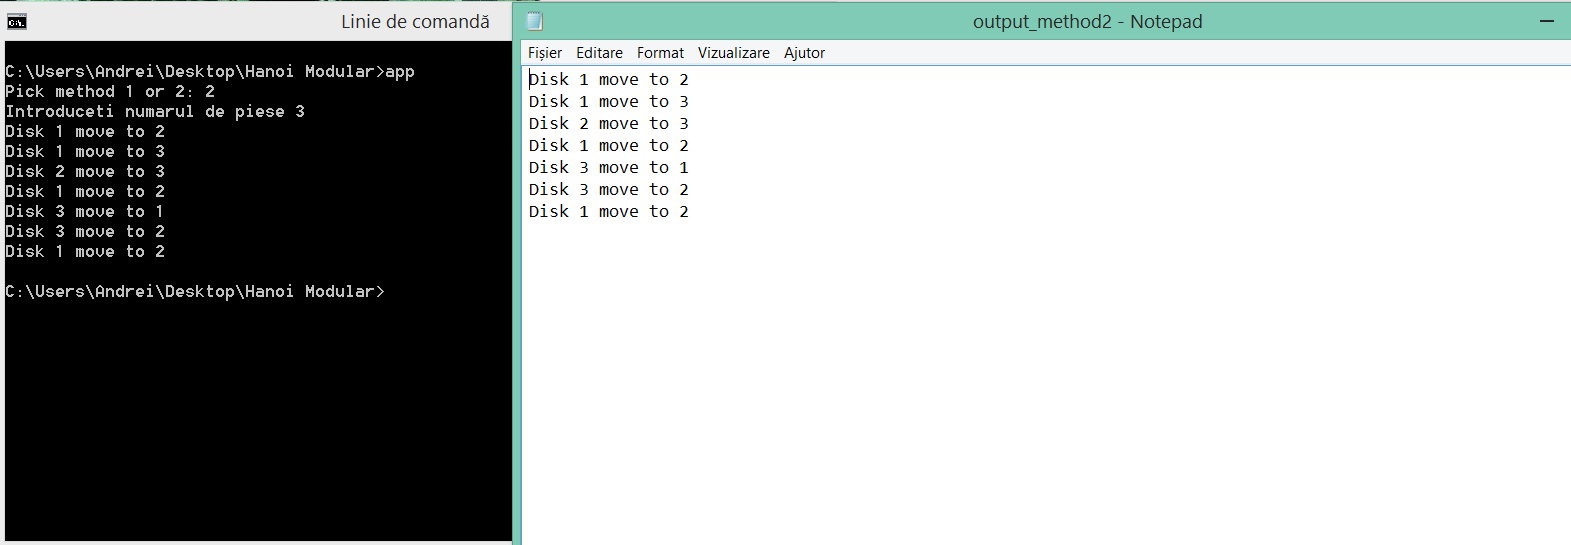
\includegraphics[scale=0.4]{metoda2.png}

\newpage
\section{Conclusion}

This program depends very much of the number of the plates introduced by the user. If we will have a number of towers larger than 15 the execution time will be bigger

\newpage
\section{References}

\textbf{Book}:

Name : Totul despre C si C++ 

Year of publication  :2005

Publisher :Teora

Author :Dr. Kris Jamsa Lars Klander\\
\textbf{Web references}:

$1.http://www.geeksforgeeks.org$

$2. https://www.sharelatex.com/learn/Main_Page$\\
\textbf{Article}:

$1.https://divideetimpera.wikispaces.com/Turnurile+din+Hanoi$


\end{document}

\section{Conclusion}
 \citep{adams1995hitchhiker}

\bibliographystyle{plain}
\bibliography{references}
\end{document}
